
% This LaTeX was auto-generated from an M-file by MATLAB.
% To make changes, update the M-file and republish this document.

\documentclass{article}
\usepackage{graphicx}
\usepackage{color}

\sloppy
\definecolor{lightgray}{gray}{0.5}
\setlength{\parindent}{0pt}

\begin{document}

    
    
\subsection*{Contents}

\begin{itemize}
\setlength{\itemsep}{-1ex}
   \item First, Load and Parse Observation Data
   \item Pre-Allocations
   \item Initialize Variables
   \item Perform Batch Loop
   \item Display Outputs
\end{itemize}
\begin{verbatim}
% function Xstar0 = BatchProcess()
% Compute new xhat
% Looks for functions to return:
%   G
%   Htilde
% Inside of /Filters/BatchTools.m

clc; clear all;close all; format compact;tic
warning off MATLAB:nearlySingularMatrix
\end{verbatim}


\subsection*{First, Load and Parse Observation Data}

\begin{verbatim}
load('Observations.mat');
t_obs       = obs(:,1);
station     = obs(:,2);
rho_obs     = obs(:,3);
rhodot_obs  = obs(:,4);
\end{verbatim}


\subsection*{Pre-Allocations}

\begin{verbatim}
x       = zeros(length(obs));
y       = x;
z       = x;
xdot    = x;
ydot    = x;
zdot    = x;
Xsite1  = x;
Ysite1  = x;
Zsite1  = x;
Xsite2  = x;
Ysite2  = x;
Zsite2  = x;
Xsite3  = x;
Ysite3  = x;
Zsite3  = x;
Phi     = cell(1,length(obs));
y_res   = zeros(2,length(obs));
Xsite   = x;
Ysite   = x;
Zsite   = x;
theta   = x;
\end{verbatim}


\subsection*{Initialize Variables}

\begin{verbatim}
% Calculations for rho, rhodot. Put into bigger functiom sometime
%---------------------------------------------
findrhostar      = @(x,y,z,Xsite,Ysite,Zsite,theta) sqrt(x^2+y^2+z^2+Xsite^2+Ysite^2+Zsite^2-2*(x*Xsite+y*Ysite)*cos(theta)+2*(x*Ysite-y*Xsite)*sin(theta)-2*z*Zsite);
findrhodotstar   = @(x,y,z,xdot,ydot,zdot,Xsite,Ysite,Zsite,theta,theta_dot,rho) (x*xdot + y*ydot + z*zdot - (xdot*Xsite + ydot*Ysite)*cos(theta) + theta_dot*(x*Xsite + y*Ysite)*sin(theta)...
                    +(xdot*Ysite - ydot*Xsite)*sin(theta) + theta_dot*(x*Ysite - y*Xsite)*cos(theta) - zdot*Zsite)...
                                                    /rho;
%---------------------------------------------

% System Constants
%---------------------------------------------
Phi_Init    = eye(18,18);
tol         = 1e-13;
uE          = 3.986004415e14;        % m^3/s^2
J2          = 1.082626925638815e-3;  % []
Cd          = 2;                     % []
theta_dot   = 7.29211585530066e-5;   % rad/s
time        = t_obs;
%---------------------------------------------

% Information
%---------------------------------------------
sigma_rho   = 0.01;                  % rms std
sigma_rhodot= 0.001;                 % rms std
R           = [sigma_rho^2  ,         0        ; ...
                    0       ,    sigma_rhodot^2];
W = inv(R);
Pbar0       = diag([1e6,1e6,1e6,1e6,1e6,1e6,1e20,1e6,1e6,1e-10,1e-10,1e-10,1e6,1e6,1e6,1e6,1e6,1e6]);
%---------------------------------------------

% Initial Conditions
%---------------------------------------------
RV_Init     = [757700,5222607.0,4851500.0,2213.21,4678.34,-5371.30];
Station_Init= [-5127510.0 , -3794160.0 , 0.0 ,...               %101
                3860910.0 , 3238490.0  , 3898094.0 , ...        %337
                549505.0  , -1380872.0 , 6182197.0 ];           %394
Const_Init = [uE , J2 , Cd ];
%---------------------------------------------

% Form Initialization State
%---------------------------------------------
Xstar0 = [RV_Init , Const_Init , Station_Init , reshape(Phi_Init,1,length(Phi_Init)^2)]';
%---------------------------------------------

% Initial xbar0, or a-priori state deviation from reference trajectory
%---------------------------------------------
xbar0       = zeros(18,1);
%---------------------------------------------
\end{verbatim}


\subsection*{Perform Batch Loop}

\begin{verbatim}
num_iterations = 1;
for ii = 1:num_iterations

    % Dynamical Integration
    %---------------------------------------------
    tol_mat     = ones(size(Xstar0)) .* tol;
    options     = odeset('RelTol',tol,'AbsTol',tol,'OutputFcn',@odetpbar);

    [time,StatePhi] = ode45(@StateDeriv_WithPhi,time,Xstar0,options);
    %---------------------------------------------


        % Batch Processing Part
    %---------------------------------------------
    Lam = inv(Pbar0);
    N   = Pbar0\xbar0;  % same as inv(pobar)*xbar0
    N_orig = N;
    Lam_orig=Lam;


    % Reform Phi Matrix
    %---------------------------------------------
    for jj = 1:length(time)
           Phi      = reshape(StatePhi(jj,19:end),size(Phi_Init));
           Xstar    = StatePhi(:,1:18);
           x        = Xstar(:,1);
           y        = Xstar(:,2);
           z        = Xstar(:,3);
           xdot     = Xstar(:,4);
           ydot     = Xstar(:,5);
           zdot     = Xstar(:,6);
           Xsite1   = Xstar(:,10);
           Ysite1   = Xstar(:,11);
           Zsite1   = Xstar(:,12);
           Xsite2   = Xstar(:,13);
           Ysite2   = Xstar(:,14);
           Zsite2   = Xstar(:,15);
           Xsite3   = Xstar(:,16);
           Ysite3   = Xstar(:,17);
           Zsite3   = Xstar(:,18);

    %---------------------------------------------





%     parfor jj = 1:length(rho_obs)
        theta(jj)          = theta_dot*time(jj);
        Htilde             = zeros(2,18);
        % Check Stations
        %---------------------------------------------
        %Station 1
        if station(jj) == 101
            Xsite(jj)   = Xsite1(jj);   Ysite(jj)=Ysite1(jj);   Zsite(jj)=Zsite1(jj);
            % Find H Tilde
            %---------------------------------------------
            Htilde = FindHtilde(Xsite(jj),Ysite(jj),Zsite(jj),theta(jj),theta_dot,x(jj),xdot(jj),y(jj),ydot(jj),z(jj),zdot(jj));
            %---------------------------------------------
            Htilde  = [Htilde , zeros(2,6)];

        end

        %Station 2
        if station(jj) == 337
            Xsite(jj)   = Xsite2(jj);   Ysite(jj)=Ysite2(jj);   Zsite(jj)=Zsite2(jj);
            % Find H Tilde
            %---------------------------------------------
            Htilde = FindHtilde(Xsite(jj),Ysite(jj),Zsite(jj),theta(jj),theta_dot,x(jj),xdot(jj),y(jj),ydot(jj),z(jj),zdot(jj));
            %---------------------------------------------
            Htilde  = [Htilde(:,1:9) , zeros(2,3), Htilde(:,10:12),zeros(2,3)];
        end

        %Station 3
        if station(jj) == 394
            Xsite(jj)   = Xsite3(jj);   Ysite(jj)=Ysite3(jj);   Zsite(jj)=Zsite3(jj);
            % Find H Tilde
            %---------------------------------------------
            Htilde = FindHtilde(Xsite(jj),Ysite(jj),Zsite(jj),theta(jj),theta_dot,x(jj),xdot(jj),y(jj),ydot(jj),z(jj),zdot(jj));
            %---------------------------------------------
            Htilde  = [Htilde(:,1:9),zeros(2,6),Htilde(:,10:12)];
        end
        %---------------------------------------------

        % Map To Epoch
        %---------------------------------------------
        H{jj}    = Htilde*Phi;
        %---------------------------------------------

        % Cumulate INFORMATION?? Matrix
        %---------------------------------------------
        Lam       = Lam + H{jj}'*W*H{jj};
        %---------------------------------------------

        % Put into FindG
        %---------------------------------------------
        rhostar   = findrhostar(x(jj),y(jj),z(jj),Xsite(jj),Ysite(jj),Zsite(jj),theta(jj));
        rhodotstar= findrhodotstar(x(jj),y(jj),z(jj),xdot(jj),ydot(jj),zdot(jj),Xsite(jj),Ysite(jj),Zsite(jj),theta(jj),theta_dot,rhostar);
        %---------------------------------------------

        % Find Observation Deviations
        %---------------------------------------------
        ystar       = [rhostar;rhodotstar];
        y_res(:,jj) = [rho_obs(jj);rhodot_obs(jj)] - ystar;
        %---------------------------------------------


        % Cumulate SOMETING?? Matrix
        %---------------------------------------------
        N     = N + H{jj}'*W*y_res(:,jj);
        %---------------------------------------------
    end
    fprintf('RMS of rho is :  %3.5f \n',rms(y_res(1,:)))
    fprintf('RMS of rhodot is :  %3.5f \n',rms(y_res(2,:)))
    % Find New State Deviation
    %---------------------------------------------
    xhat0   = Lam\(N);
    %---------------------------------------------

    % Update Best Guess of Initial Conditions
    %---------------------------------------------
    Xstar0  = [Xstar0(1:18) + xhat0; (reshape(Phi_Init,length(Phi_Init)^2,1))];
    %---------------------------------------------

    % Update a-priori State Deviation
    %---------------------------------------------
    xbar0 = xbar0 - xhat0;
    %---------------------------------------------


    figure(1)
    subplot(num_iterations,2,2*ii-1)
    plot(y_res(1,:))
    ylabel('rho residules')
    xlabel('observation number')

    subplot(num_iterations,2,2*ii)
    plot(y_res(2,:))
    ylabel('rho residules')
    xlabel('observation number')

end

fprintf('\n\nRunning Time for Batch Processor : %3.5f\n\n',toc)
\end{verbatim}

        \color{lightgray} \begin{verbatim}ODE integration: 100%    [..........]
   Integration time: 3.1912
RMS of rho is :  732.74831 
RMS of rhodot is :  2.90017 


Running Time for Batch Processor : 4.44755

\end{verbatim} \color{black}
    
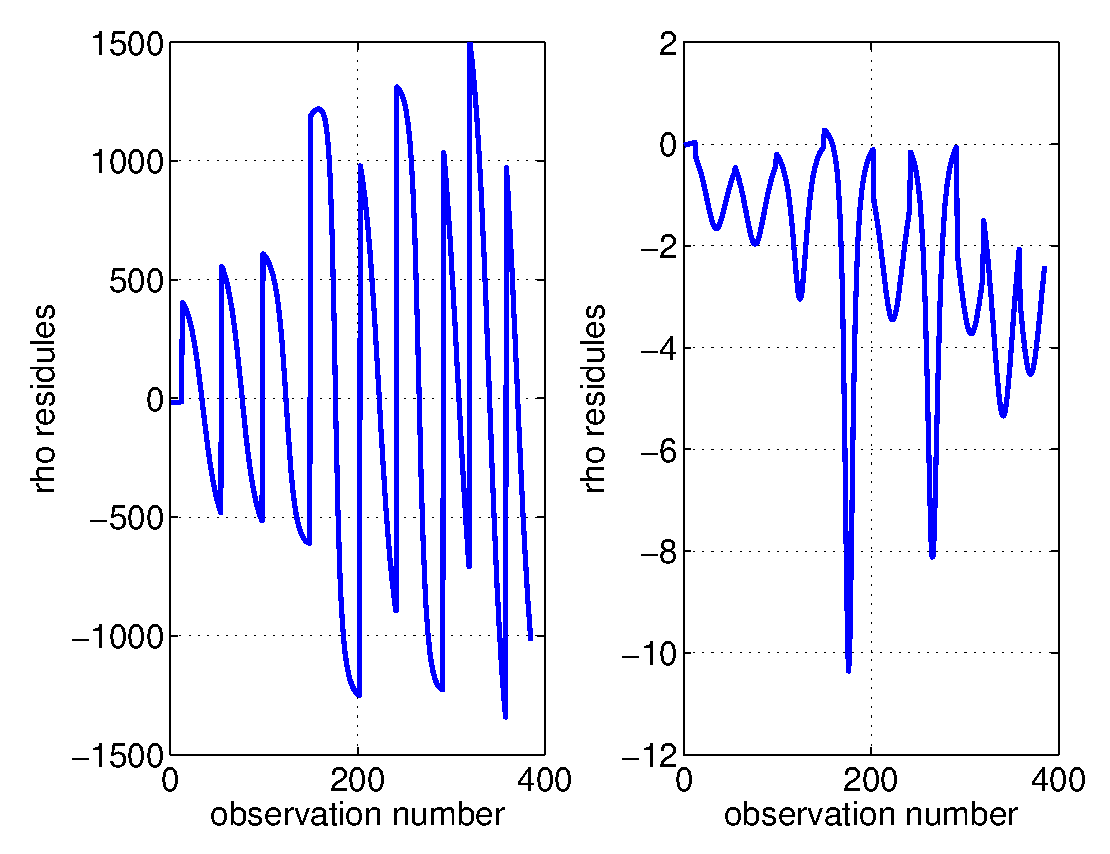
\includegraphics [width=4in]{BatchProcess_01.eps}


\subsection*{Display Outputs}

\begin{verbatim}
SumHtWH = Lam - Lam_orig;
SumHtWy = N - N_orig;

fprintf('Sum of H''WH is :\n')
printMatrix(SumHtWH,27,10);
fprintf('\n\n\n Sum of H''Wy is :\n')
printMatrix(SumHtWy,15,5);

fprintf('\n\n\n Output of xhat0 is :\n')
printMatrix(xhat0,27,10)
\end{verbatim}

        \color{lightgray} \begin{verbatim}Sum of H'WH is :
        15642892.2139638532	        96445342.0481109023	        87553862.2093564719	     39035426229.8915863037	     85380621054.4556427002	    -89456061116.4034271240	              -1.5954227562	 286051153800621.4375000000	        -7713897.2730123671	           94424.1960645709	          -55744.7939965413	         1837092.6939293954	          678092.1290839665	          638409.6495227553	        -1277860.1201436382	          733971.6775837080	          635723.5618613327	          123510.5898856849	
        96445342.0481109023	       647567086.6741099358	       591096262.6015053988	    261992453682.0038146973	    568653301031.6795654297	   -602809745181.2003173828	             -10.7016510482	1995728895595858.5000000000	       -52282664.0776869431	         -773424.0039953113	         1432595.0899111021	        10595645.8622289877	         7392018.3361077625	         1308575.5194160349	        -8711564.5189841464	         6309531.7304992266	         1145230.3956329017	         -266474.1940985713	
        87553862.2093564868	       591096262.6015053988	       545069191.1156791449	    239589749865.7162170410	    517506233589.1514892578	   -554569933689.5238037109	              -9.8035792463	1834580284670072.5000000000	       -48506619.6265168786	         -402655.1210385546	         1045048.6870896441	         8376683.0559452018	         7194081.2672169982	         1587982.6929616374	        -8729815.9775514472	         6065287.8468057951	         1084368.6505893399	         -273346.3020820002	
     39035426229.8915939331	    261992453682.0038452148	    239589749865.7162170410	 106661554804651.4062500000	 230019289585374.4687500000	-244305773049970.0625000000	           -4332.9515060860	803726582978524416.0000000000	    -21168772678.9310188293	       -50859313.7735307217	       302043238.1972026825	      4288498976.4752812386	      2916254082.3784904480	       611717806.8690390587	     -3472182365.3918185234	      2884955908.2518606186	       206458670.4745006561	      -225374609.3335765600	
     85380621054.4556274414	    568653301031.6795654297	    517506233589.1514892578	 230019289585374.4687500000	 500449734561211.2500000000	-528426575793172.3750000000	           -9393.3837935608	1745988440697024256.0000000000	    -45491258336.3640747070	      -690061915.6090250015	      1311456344.9984645844	      9736126092.6784706116	      6209844895.7019824982	      1224063166.9970550537	     -7345835814.4685678482	      5408488696.8719940186	      1469890745.0940928459	       -83278163.7571291327	
    -89456061116.4034271240	   -602809745181.2001953125	   -554569933689.5236816406	-244305773049970.0625000000	-528426575793172.3125000000	 564925217977991.5000000000	            9992.9746072029	-1868777680042144768.0000000000	     49351823593.8733901978	       453804529.4006270766	     -1186627512.8099844456	     -8815559900.1859703064	     -7155118427.5747156143	     -1442785596.3882243633	      8473696896.6845960617	     -6211919135.8050832748	     -1275868107.9849932194	       227040169.4953751564	
              -1.5954227562	             -10.7016510482	              -9.8035792463	           -4332.9515060860	           -9393.3837935608	            9992.9746072029	               0.0000001772	       -33071416.4047614485	               0.8680775739	               0.0105353831	              -0.0212645324	              -0.1670443062	              -0.1240245340	              -0.0250132771	               0.1466430480	              -0.1057804599	              -0.0238949898	               0.0031677740	
 286051153800621.4375000000	1995728895595858.5000000000	1834580284670072.5000000000	803726582978524544.0000000000	1745988440697024000.0000000000	-1868777680042144512.0000000000	       -33071416.4047614485	6357520838113366114304.0000000000	-162933815454797.0937500000	  -5176617560516.4169921875	   8224474829224.8125000000	  27349691260043.2031250000	  27574275176521.5312500000	     81037364953.2355957031	 -27206535197374.7304687500	  19159599168762.6289062500	   3598318516081.8442382812	   -805207179437.5408935547	
        -7713897.2730123661	       -52282664.0776869431	       -48506619.6265168637	    -21168772678.9310188293	    -45491258336.3640747070	     49351823593.8733901978	               0.8680775739	-162933815454797.1250000000	         4712675.9088873239	            4607.5040727804	          -47211.4081440844	         -617765.3808566579	         -571670.9101045745	          -87065.8866727704	          691156.4551380392	         -593635.2690462477	           36198.6465750722	           59945.3954439472	
           94424.1960645709	         -773424.0039953114	         -402655.1210385547	       -50859313.7735307217	      -690061915.6090250015	       453804529.4006271362	               0.0105353831	  -5176617560516.4169921875	            4607.5040727804	          301411.2586326599	         -238883.2131691568	           13355.2193051041	               0.0000000000	               0.0000000000	               0.0000000000	               0.0000000000	               0.0000000000	               0.0000000000	
          -55744.7939965413	         1432595.0899111023	         1045048.6870896443	       302043238.1972027421	      1311456344.9984645844	     -1186627512.8099844456	              -0.0212645324	   8224474829224.8115234375	          -47211.4081440844	         -238883.2131691568	          382196.5541191101	           -5925.9028849073	               0.0000000000	               0.0000000000	               0.0000000000	               0.0000000000	               0.0000000000	               0.0000000000	
         1837092.6939293954	        10595645.8622289877	         8376683.0559452018	      4288498976.4752812386	      9736126092.6784706116	     -8815559900.1859703064	              -0.1670443062	  27349691260043.2031250000	         -617765.3808566579	           13355.2193051041	           -5925.9028849073	          547491.3019981384	               0.0000000000	               0.0000000000	               0.0000000000	               0.0000000000	               0.0000000000	               0.0000000000	
          678092.1290839666	         7392018.3361077616	         7194081.2672169982	      2916254082.3784904480	      6209844895.7019824982	     -7155118427.5747156143	              -0.1240245340	  27574275176521.5351562500	         -571670.9101045745	               0.0000000000	               0.0000000000	               0.0000000000	          443985.4002217269	         -187039.8461420266	         -202932.9174915103	               0.0000000000	               0.0000000000	               0.0000000000	
          638409.6495227553	         1308575.5194160349	         1587982.6929616374	       611717806.8690390587	      1224063166.9970550537	     -1442785596.3882243633	              -0.0250132771	     81037364953.2366943359	          -87065.8866727704	               0.0000000000	               0.0000000000	               0.0000000000	         -187039.8461420266	          489429.5398828702	         -185546.2470719735	               0.0000000000	               0.0000000000	               0.0000000000	
        -1277860.1201436382	        -8711564.5189841483	        -8729815.9775514472	     -3472182365.3918190002	     -7345835814.4685678482	      8473696896.6845960617	               0.1466430480	 -27206535197374.7382812500	          691156.4551380392	               0.0000000000	               0.0000000000	               0.0000000000	         -202932.9174915103	         -185546.2470719735	          467743.5986754843	               0.0000000000	               0.0000000000	               0.0000000000	
          733971.6775837080	         6309531.7304992266	         6065287.8468057951	      2884955908.2518606186	      5408488696.8719940186	     -6211919135.8050832748	              -0.1057804599	  19159599168762.6289062500	         -593635.2690462477	               0.0000000000	               0.0000000000	               0.0000000000	               0.0000000000	               0.0000000000	               0.0000000000	          477457.6594665953	         -145787.8075451687	          -99770.1215443975	
          635723.5618613327	         1145230.3956329024	         1084368.6505893404	       206458670.4745006561	      1469890745.0940928459	     -1275868107.9849936962	              -0.0238949898	   3598318516081.8452148438	           36198.6465750722	               0.0000000000	               0.0000000000	               0.0000000000	               0.0000000000	               0.0000000000	               0.0000000000	         -145787.8075451687	          666808.3371934118	          208656.0639778854	
          123510.5898856849	         -266474.1940985713	         -273346.3020820001	      -225374609.3335765600	       -83278163.7571291327	       227040169.4953751564	               0.0031677740	   -805207179437.5407714844	           59945.3954439472	               0.0000000000	               0.0000000000	               0.0000000000	               0.0000000000	               0.0000000000	               0.0000000000	          -99770.1215443974	          208656.0639778854	           76408.2371207681	



 Sum of H'Wy is :
5486061547.19810	
36584442778.58514	
33408872159.34251	
14834824166248.30859	
32158626582387.25391	
-34086624652357.96484	
     -604.98783	
112317807659114768.00000	
-2948644630.17576	
-27771434.44241	
 67040528.11551	
603470756.22806	
400176817.76198	
 91700586.30273	
-484097205.11321	
369071814.20939	
 75465589.38682	
-13494689.60293	



 Output of xhat0 is :
              -0.0363025898	
              -0.2741066153	
              -0.1808766575	
               0.0409349622	
               0.0327483949	
              -0.0147530394	
        -9463442.1830325481	
              -0.0000006574	
               0.1475547229	
               0.0000018632	
               0.0000013787	
              -0.0000002538	
             -10.5636296834	
               9.9833774037	
               5.7943247874	
              -5.7819128352	
               2.3443688041	
               1.5124575876	
\end{verbatim} \color{black}
    


\end{document}
    
